\let\negmedspace\undefined
\let\negthickspace\undefined
\documentclass[journal]{IEEEtran}
\usepackage[a5paper, margin=10mm, onecolumn]{geometry}
%\usepackage{lmodern} 
\usepackage{tfrupee} 

\setlength{\headheight}{1cm} 
\setlength{\headsep}{0mm}     

\usepackage{gvv-book}
\usepackage{gvv}
\usepackage{cite}
\usepackage{amsmath,amssymb,amsfonts,amsthm}
\usepackage{algorithmic}
\usepackage{graphicx}
\usepackage{textcomp}
\usepackage{xcolor}
\usepackage{txfonts}
\usepackage{listings}
\usepackage{enumitem}
\usepackage{mathtools}
\usepackage{gensymb}
\usepackage{comment}
\usepackage[breaklinks=true]{hyperref}
\usepackage{tkz-euclide} 
\usepackage{listings}                                        
\def\inputGnumericTable{}                                 
\usepackage[latin1]{inputenc}                                
\usepackage{color}                                            
\usepackage{array}                                            
\usepackage{longtable}                                       
\usepackage{calc}                                             
\usepackage{multirow}                                         
\usepackage{hhline}                                           
\usepackage{ifthen}                                           
\usepackage{lscape}

\begin{document}

\bibliographystyle{IEEEtran}
\vspace{3cm}

\title{1.11.5}
\author{AI25BTECH11003 - Bhavesh Gaikwad}
{\let\newpage\relax\maketitle}

\renewcommand{\thefigure}{\theenumi}
\renewcommand{\thetable}{\theenumi}
\setlength{\intextsep}{10pt} 


\numberwithin{equation}{enumi}
\numberwithin{figure}{enumi}
\renewcommand{\thetable}{\theenumi}


\textbf{Question}: The scalar product of vector $\overrightarrow{a} = \hat{i} + \hat{j} + \hat{k}$ with a unit vector along the sum of the vectors $\overrightarrow{b} =2\hat{i} + 4\hat{j} - 5\hat{k}$ and $\overrightarrow{c} = \lambda\hat{i} + 2\hat{j} + 3\hat{k}$ is equal to 1. Find the value of $\lambda$ and hence find the unit vector along $\overrightarrow{b} + \overrightarrow{c}$. \\\\

\textbf{Solution:}\\

 Given: $\vec{a}=\myvec{1\\1\\1}$,  $\vec{b}=\myvec{2\\4\\-5}$,  $\vec{c}=\myvec{\lambda\\2\\3}.$

Let $\vec{u}$ be the unit vector along $\vec{b} + \vec{c} .$ \\

$ \vec{b} + \vec{c} = \myvec{2+\lambda\\4+2\\-5+3}
=\myvec{2+\lambda\\6\\-2}.$ \\

$\|\vec{b}+\vec{c}\| = \sqrt{(2+\lambda)^2+6^2+(-2)^2}
 = \sqrt{\lambda^2+4\lambda+44}.$ \\

$\vec{u}$ = $\dfrac{\vec{b} + \vec{c}}{\|\vec{b}+\vec{c}\|}$ = $\dfrac{1}{\sqrt{\lambda^2+4\lambda+44}} \myvec{2+\lambda\\6\\-2}.$ \\\\


Given condition: $\vec{a}\cdot \vec{u}=1.$  

$$ \vec{a}\cdot\vec{u} = \dfrac{\vec{a}\cdot(\vec{b}+\vec{c})}{\|\vec{b}+\vec{c}\|}
= \dfrac{\myvec{1\\1\\1}\cdot\myvec{2+\lambda\\6\\-2}}
{\sqrt{\lambda^2+4\lambda+44}}
= \dfrac{\lambda+6}{\sqrt{\lambda^2+4\lambda+44}}=1.
$$ \\


$
\Rightarrow\ (\lambda+6)^2=\lambda^2+4\lambda+44
\ \Longrightarrow\ 
\lambda^2+12\lambda+36=\lambda^2+4\lambda+44
\ \Longrightarrow\ 
8\lambda=8\ $
$$\Longrightarrow\ 
\boxed{\lambda=1}$$

Now, with $\lambda=1:\quad \vec{b}+\vec{c}
=\myvec{3\\6\\-2},\quad \|\vec{b}+\vec{c}\|
=\sqrt{3^2+6^2+(-2)^2} = \sqrt{49} = 7.$ \\

Unit vector along, $\vec{b}+\vec{c}$ is: $\quad \dfrac{1}{7}\myvec{3\\6\\-2}
= \dfrac{1}{7}\myvec{3\\6\\-2}.$\\\\
\bigskip
\begin{align}   
\centering
\boxed{\lambda=1} \quad and \qquad 
\boxed{\text{Unit vector along }\,\vec{b}+\vec{c}
=\dfrac{1}{7}\myvec{3\\6\\-2}}.
\end{align}

\bigskip

\begin{figure}[htbp]
    \centering
    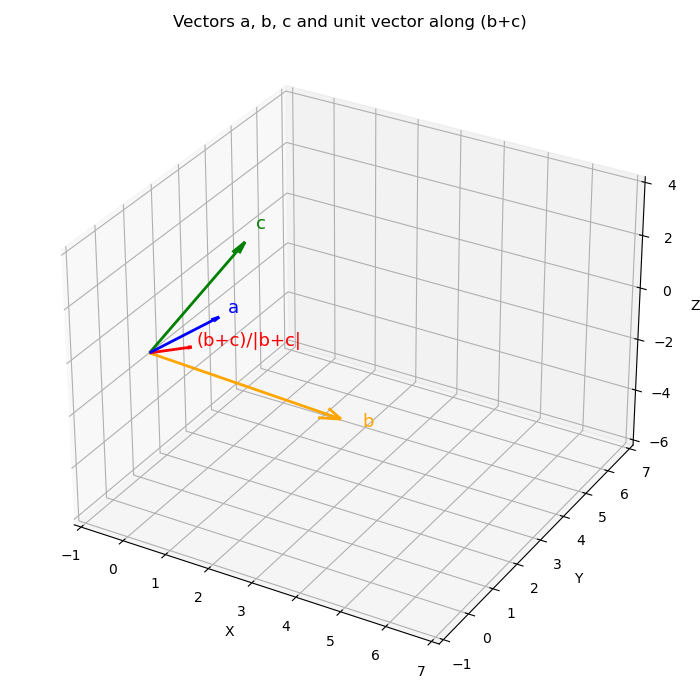
\includegraphics[width=0.8\linewidth]{figs/fig1.png}
    \caption{Vector Representation}
    \label{fig:fig/fig1.png}
\end{figure}
\end{document}  
